The environment used is build with Unity as a set of obstacles with all of edges either perpendiculars or parallels.

In order to enhance the performance, we discretize our environment using a grid. Each cell is either \emph{occupied} if one of its corners lies into an obstacle or \emph{free}.

The environment is then covered by a set of convex $C_{1\leq i \leq n}$ with each $C_i$ satisfying the following criteria.

\begin{criteria}[of Visibility]
 \emph{For all point $P$ in the area, if each corner of $C_i$ is visible, then the whole area is visible}. In practice, it means that checking if a convex can be seen from a given point can be done in only $4$ raycasting.
\label{visibilityCriteria}
\end{criteria}

The three problems we investigate involve finding interesting point on the map. We uses the following denomination:
\begin{description}
	\item[Waypoints:] Points at a given distance of each obstacle corners (see Figure \ref{convexCover});
	\item[Points of surveillance:] Points from which all the area is surveyed.
\end{description}

\subsection{Convex set cover}

In order to solve our three problems, we needed a convex cover set of our area. The algorithm used to create the convex set is based on the work from \cite{CoopMinTime}. Figure \ref{convexCover} shows the convex cover generated by the algorithm \ref{algoConvexCover}.

\begin{algorithm}
This algorithm describe how to create a maximal convex cover of our environment. Since the obstacles are all orthogonal, the maximal convex sets $C_i$ is rectangles aligned with the polygons.
\begin{enumerate}
\item Based on the grid, make a discretization of the environment $G(A)$.
\item Find a yet uncovered cell, p.
\item Start growing a rectange $C_i$ from $p$ until it's length and/or width reach $R$\footnote{R is the maximum convex size in width and/or length. This parameter is used to guarantee the visibily criteria \ref{visibilityCriteria}}.
\item While uncovered cells exists, goto 2.
\end{enumerate}
\label{algoConvexCover}
\end{algorithm}

\begin{figure}[h!t]
	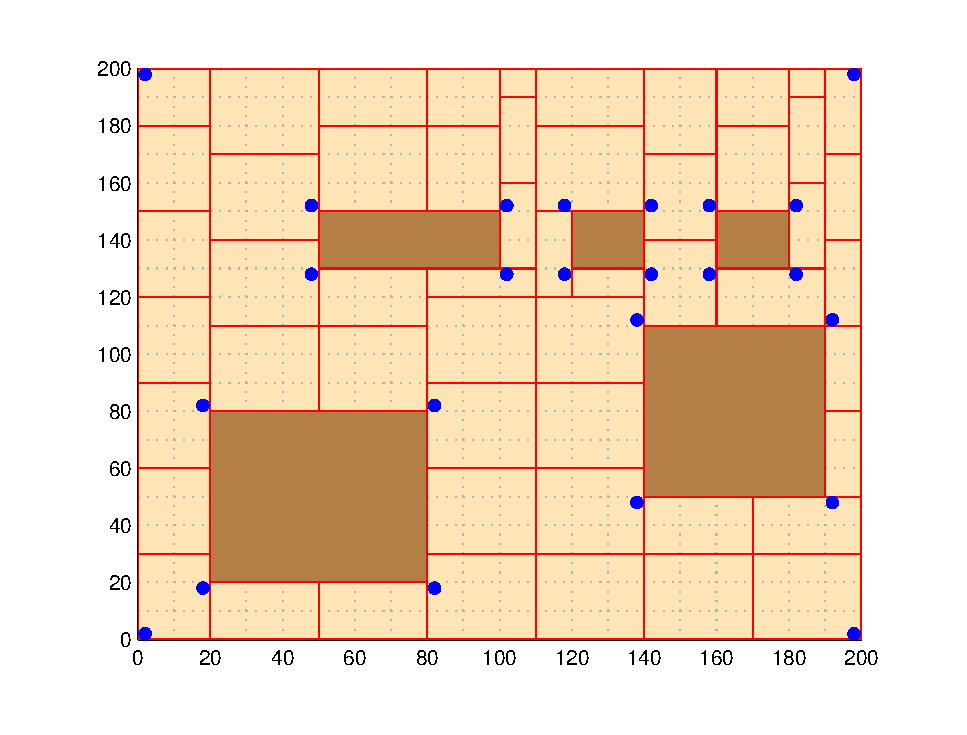
\includegraphics[width=\linewidth]{fig/convexCover.eps}
	\caption{Waypoints of the environment \& Convex set cover}
	\label{convexCover}
\end{figure}


\subsection{Graph representation \& search}

\textsc{About graph generation from the environment using waypoints and the $A^{\ast}$ algorithm!}
